\documentclass[12pt]{article}

\topmargin -40pt
\marginparwidth 0pt
\oddsidemargin  -40pt
\evensidemargin 0pt
\marginparsep 0pt
\textwidth 7.2 in
\textheight  10 in
\hoffset  0.1in
\linespread{1.3}

\usepackage{amsthm,amsmath,amssymb,amscd,verbatim,epsfig}
\usepackage{mathptmx}
\usepackage{amsfonts}
%\usepackage{setapace}
\usepackage{graphicx}
\usepackage{bm}
%\usepackage{CJK}
\usepackage{ulem}
\usepackage{multicol}
\usepackage{enumerate}
\usepackage{float}
\usepackage{fontspec}
\usepackage{xeCJK}
\usepackage{graphicx}
\usepackage{multicol}
\usepackage{array}

\setmainfont{Times New Roman}
\setCJKmainfont{TaipeiSansTCBeta-Regular}
\XeTeXlinebreaklocale "zh"
\XeTeXlinebreakskip = 0pt plus 1pt

\title{Homework 2 of Computational Mathematics}
\author{AM15 黃琦翔 111652028}

\begin{document}
\maketitle
\begin{enumerate}
    \item $x^3 = x + 1\implies x^2 = 1 + \dfrac{1}{x}\implies x = \sqrt{1 + \dfrac{1}{x}} = g(x)$.
    $p_1 = g(p_0) = \sqrt{1 + 1} = \sqrt{2} \approx 1.414$.
    $p_2 = g(p_1) = \sqrt{1 + \dfrac{1}{\sqrt{2}}} \approx 1.3065$.
    $p_3 = g(p_2) \approx 1.3172$.
    $p_4 = g(p_3) \approx 1.326$.
    $p_5 = g(p_4) \approx 1.324$ 
    Then, $p_4$ is the answer that we want to find.

    \item Let $f(x) = x^3 + x - 4$, $f'(x) = 3x^2 + 1 < 49$ for all $x\in [1, 4]$.
    Thus, for $|x - y| < \dfrac{10^{-3}}{49} \approx 2.0409e-5$, $|f(x) - f(y)| < 10^3$.
    Find $n$ s.t. $3 \cdot 2^{-n} < 2.0409e-5$, $n > -\log_2(\dfrac{2.0409e-5}{3}) \approx 17.1653$.
    Thus, the bound of the number of iteration is $18$.
    Then, by python code below, the root is about $1.3787$.

    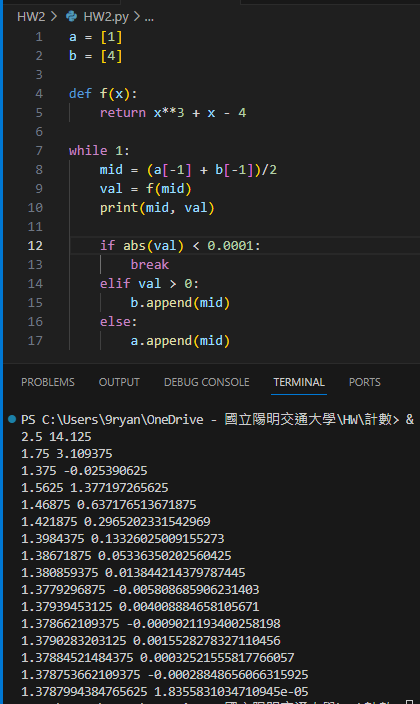
\includegraphics[scale = 0.6]{2024-03-22-214359}

    \item In this question, we let $p_{n+1} = g(p_n)$ and $p = \sqrt[3]{21}$.
    And by $\displaystyle\lim_{n\to\infty} \dfrac{|p_{n+1} - p|}{|p_n - p|^\alpha} = \lambda$, 

    $\dfrac{|p_{n+1}-p|}{|p_n-p|} \approx \dfrac{\lambda |p_n-p|^\alpha}{\lambda |p_{n-1}-p|^\alpha} \approx \left|\dfrac{p_n - p}{p_{n-1}-p}\right|^\alpha$,
    then $\alpha \approx \dfrac{\ln |(p_{n+1} - p)/(p_n - p)|}{\ln |(p_n-p)/(p_{n-1}-p)|}$.
    
    Then, by observing the function, we get b is quadratic convergence (Newton's method).
    In the meanwhile, though $\sqrt[3]{21}$ is a fixed point of c, but it will diverges or converges to $0$ for any open interval contains $\sqrt[3]{21}$.

    Thus, by result of iteration with python below, the order of speed of convergence is b > d > a.

    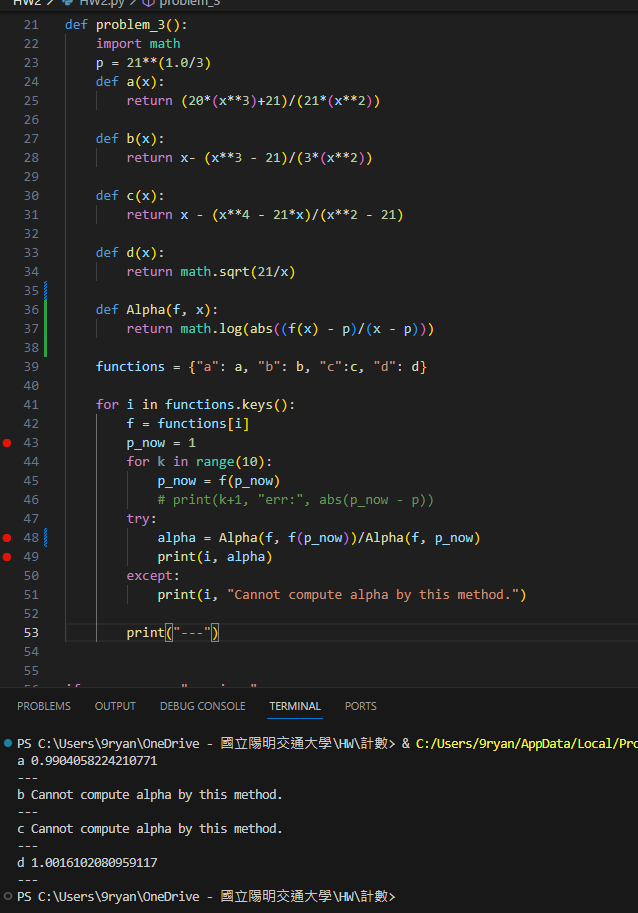
\includegraphics[scale = 0.7]{2024-03-24-204951.png}

    \item $|g'(x)| = |-2^{-x}\ln(2)|$ is continuous and decreasing on $\mathbb{R}$.
    Thus, $g'(\dfrac{1}{3}) \approx 0.55015$.
    And since $g(\dfrac{1}{3})\approx 0.79370 > \dfrac{1}{3}$ and $g(1) = \dfrac{1}{2} < 1$.
    By Theorem 2.3, $g(x)$ has unique fixed point on $[\dfrac{1}{3}, 1]$.

    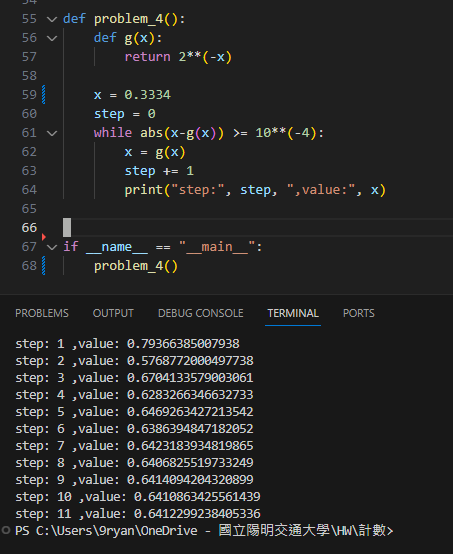
\includegraphics[scale = 0.8]{2024-03-24-211516.png}

    By the result from python above, we need $12$ steps to let error less than $10^{-4}$.
    Since $|g'(x)| \leq \ln(2)2^{-x} \leq 0.551$, we take $k = 0.551$ and $p_0 = 1$.
    $|p_n - p| \leq \dfrac{k^n}{1-k} |p_1 - p| \approx k^n\cdot 1.113585746 \leq 10^{-4}$.
    Then, $n \geq 15.633566$, that is, the bound is $16$ times of iteration.

    \item \begin{enumerate}
        \item Let $x_*$ be nonzero fixed point of $g$, $x_* = 2x_* - Ax_*^2 \implies x_* = Ax_*^2\implies x^*A = 1$.
        Thus, $x_* = \dfrac{1}{A}$.

        \item Since $g'(x) = 2 - 2Ax$ and we need $|g'(x)| < k < 1$, \begin{align*}
            |2-2Ax| < k & \iff -k < 2-2Ax < k\\
            &\iff \dfrac{k-2}{2A} < x < \dfrac{k+2}{2A}\\
            &\overset{k=1-\epsilon}{\iff} \dfrac{1}{2A} + \dfrac{\epsilon}{2A} < x < \dfrac{3}{2A} - \dfrac{\epsilon}{2A}
        \end{align*}

        Thus, $x\in \left( \dfrac{1}{2A} + \dfrac{3}{2A}\right)$.
    \end{enumerate}

    \item Let $g(x) = \dfrac{x}{2} + \dfrac{A}{2x}$, and $g'(x) = \dfrac{1}{2} - \dfrac{A}{2x^2}$.
    For $x \in (\sqrt{A}, \infty)$, $|g'(x)| \leq \dfrac{1}{2}$.
    And since $x > \sqrt{A}$, $\dfrac{x}{2} + \dfrac{A}{2x} - \sqrt{A} = \dfrac{x^2 + A -2Ax}{2x} = \dfrac{(x-\sqrt{A})^2}{2x} > 0$.
    Thus, if $x>\sqrt{A}$, $g(x) > \sqrt{A}$.
    By Corollary 2.5, $g(x)$ converges to $\sqrt{A}$ for all $(\sqrt{A}, \infty)$.

    Then, for $x\in (0, \sqrt{A})$, $\dfrac{x}{2}+\dfrac{A}{2x} - \sqrt{A} = \dfrac{(A-x)^2}{2x} > 0$.
    Thus, for $0 < x < \sqrt{A}$, $g(x) > \sqrt{A}$, and then by the argument above, it will converge to $\sqrt{A}$, too.

    Therefore, for $x_0 > 0$, $x_n$ will converge to $\sqrt{A}$.

    \item \begin{enumerate}
        \item $p_2 = p_1 - \dfrac{f(p_1)[p_0-p_1]}{f(p_0) - f(p_1)} = -\dfrac{-1}{-1+\cos(-1)-1} = \dfrac{1}{-2+\cos(1)}\approx -0.6850733573260451$.
        
        $p_3 = p_2 - \dfrac{f(p_2)[p_1 - p_2]}{f(p_1) - f(p_2)} \approx -1.252076488909229$.

        \item $p_2 = p_1 - f(p_1)\cdot \dfrac{p_0 - p_1}{f(p_0) - f(p_1)} \approx -0.6850733573260451$.
        Since $f(p_2)< 0$, $f(p_2)\cdot f(p_0)<0$.

        Then, $p_3 = p_2 - f(p_2)\cdot \dfrac{p_0 - p_2}{f(p_0) - f(p_2)} \approx -0.8413551256656522$.
    \end{enumerate}

    \item From the question, we can rewrite it as $f(i) = 1000(1 - (1+i)^{-30\cdot 12}) - 135,000i = 0$.
    After testing, we know that $f(0.002) > 0$ and $f(0.01) < 0$.

    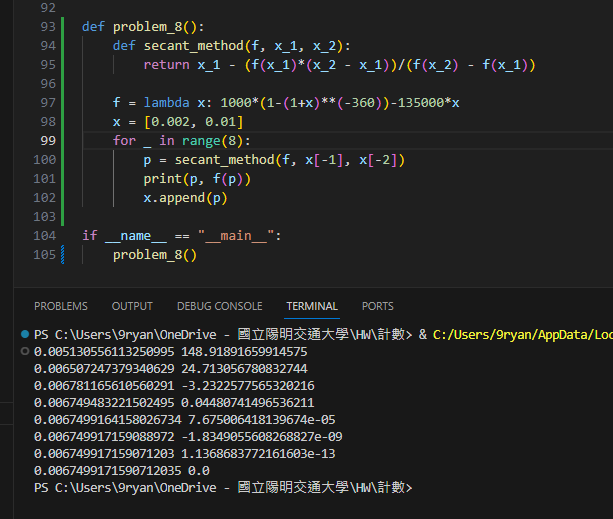
\includegraphics[scale=0.7]{2024-03-26-195318.png}

    Then, by secant method and python, $i\approx 0.0067499171590712035$.
    Thus, the interest rate the borrower can afford is about $0.0067499171590712035\cdot 12 = 0.080999005908854442 = 8.0999005908854442\%$.

    \item \begin{enumerate}
        \item $\displaystyle\lim_{n\to\infty} \dfrac{|1/(n+1)^k|}{|1/n^k|} = \displaystyle\lim_{n\to\infty} \left(\dfrac{n}{n+1}\right)^k = 1$ for all $k$.
        Thus, $p_n$ converges linearly.

        \item $\displaystyle\lim_{n\to\infty} \dfrac{10^{-2^{n+1}}}{|10^{-2^n}|^2} = \displaystyle\lim_{n\to\infty} 10^{-2^{n+1} + 2^{n}\cdot 2} = 1$.
        Thus, $p_n$ converges linearly.
    \end{enumerate}

    \item \begin{enumerate}
        \item $\ $

        \begin{center}
            \begin{tabular}{|p{1cm}|p{3cm}||p{1cm}|p{3cm}|}
                \hline
                i & $p_i$ & j & $\hat{p}_j$\\
                \hline
                0 & 0.5 & &\\
                1 & 0.8775825618 & &\\
                2 & 0.6390124941 & 0 & 0.7313851863\\
                3 & 0.8026851006 & 1 & 0.7360866917\\
                4 & 0.6947780267 & 2 & 0.7376528713\\
                5 & 0.7681958312 & 3 & 0.7384692208\\
                6 & 0.7191654459 & 4 & 0.7387980651\\
                \hline
            \end{tabular}
        \end{center}

        \item From 1., we let $g(x) = \sqrt{1 + \dfrac{1}{x}}$ and do iteration.
        
        \begin{center}
            \begin{tabular}{|c|c|c|c||c|}
                \hline
                i & $p_0$ & $p_1$ & $p_2$ & $\hat{p}_i$ \\
                \hline
                0 & 2 & 1.22474487139 & 1.34777467735 & 1.33092441907\\
                1 & 1.3309244190 & 1.32338863029 & 1.32500412497 & 1.32471893841\\
                \hline
            \end{tabular}
        \end{center}

        The answer above is given by python.

        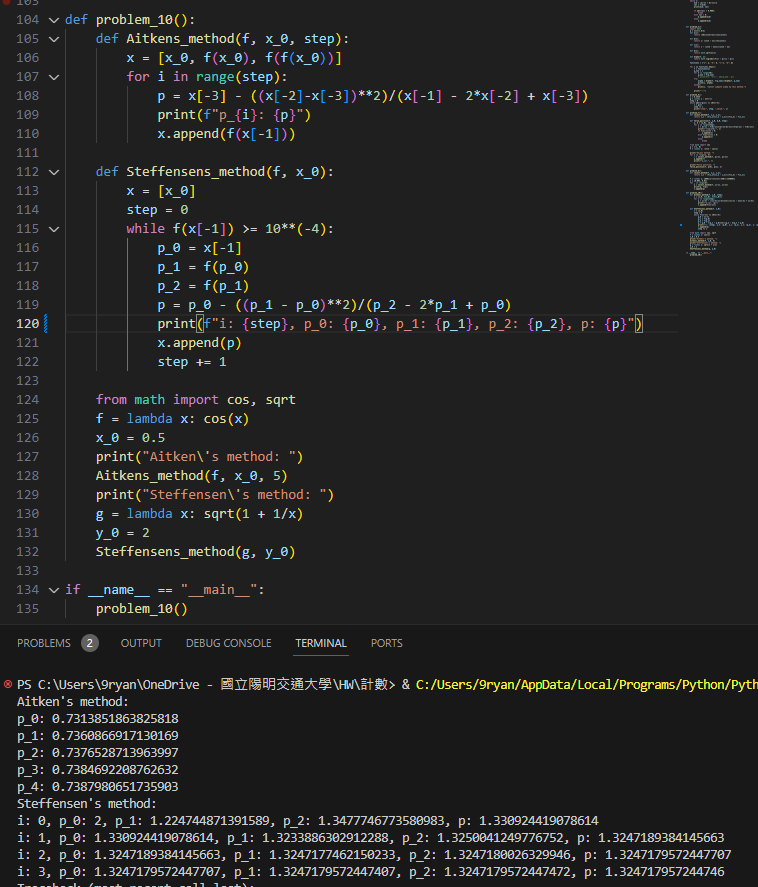
\includegraphics[scale=0.6]{2024-03-27-171617.png}
    \end{enumerate}

    \item \begin{enumerate}
        \item $\ $
        
        \begin{tabular}{|c||p{5cm}|m{5cm}|}
            \hline
            \multicolumn{3}{|c|}{$P(x) = x^3 - 5x^2 + 8x -6$, $x_0 = 2$.}\\
            \hline
            Step & y & z\\
            \hline
            0 & $a_0 = 1$ & $a_0 = 1$\\
            1 & $1 \cdot 2 - 5 = -3$ & $1 \cdot 2 + -3 = -1$\\
            2 & $-3 \cdot 2 + 8 = 2$ & $-1 \cdot 2 - 2 = 0$\\
            3 & $2 \cdot 2 - 6 = -2$ & \\
            \hline
        \end{tabular}

        Then, $P(2) = -2$ and $P'(2)=0$.

        \begin{tabular}{|c||p{5cm}|p{5cm}|}
            \hline
            \multicolumn{3}{|c|}{$P(x) = x^3 - 5x^2 + 8x -6$, $x_0 = 4$.}\\
            \hline
            Step & y & z\\
            \hline
            0 & $a_0 = 1$ & $a_0 = 1$\\
            1 & $1 \cdot 4 - 5 = -1$ & $1 \cdot 4 - 1 = 3$\\
            2 & $-1 \cdot 4 + 8 = 4$ & $3 \cdot 4 + 4 = 16$\\
            3 & $4 \cdot 4 - 6 = 10$ & \\
            \hline
        \end{tabular}

        Then, $P(4) = 10$ and $P'(4) = 16$.

        \item $P(x) = x^3 - 5x^2 + 8x -6$ and $P'(x) = 3x^2 - 10x + 8$.
        And since $P'(2) = 0$, Newton's method may not be usefully in $x_0 = 2$.
        Then, for $x_0 = 4$, 
        \begin{center}
            \begin{tabular}{|c||l|l|l|l|}
                \hline
                \multicolumn{5}{|c|}{Newton's method for $P(x)$ with $x_0 = 4$.}\\
                \hline
                i & $x_i$ & $f(x_i)$ & $f'(x_i)$ & $x_{i+1}$\\ 
                \hline
                0 & 4 & 10 & 16 & 3.375\\
                1 & 3.375 & 2.490234375 & 8.421875 & 3.07931354359925\\
                2 & 3.079313543599258 & 0.42222920359638394 & 5.65338026338887 & 3.00462739408783\\
                3 & 3.004627394087836 & 0.02322272062870922 & 5.03708339103081 & 3.00001704344919\\
                4 & 3.000017043449198 & 8.52184079072060e-05 & &\\
                \hline
            \end{tabular}
        \end{center}

        \item 
    \end{enumerate}
\end{enumerate}
\end{document}
